\documentclass[conference]{IEEEtran}
%\usepackage[backend=bibtex]{biblatex}
% Some Computer Society conferences also require the compsoc mode option,
% but others use the standard conference format.
%
% If IEEEtran.cls has not been installed into the LaTeX system files,
% manually specify the path to it like:
% \documentclass[conference]{../sty/IEEEtran}

% Some very useful LaTeX packages include:
% (uncomment the ones you want to load)

% *** MISC UTILITY PACKAGES ***
%
%\usepackage{ifpdf}
% Heiko Oberdiek's ifpdf.sty is very useful if you need conditional
% compilation based on whether the output is pdf or dvi.
% usage:
% \ifpdf
%   % pdf code
% \else
%   % dvi code
% \fi
% The latest version of ifpdf.sty can be obtained from:
% http://www.ctan.org/pkg/ifpdf
% Also, note that IEEEtran.cls V1.7 and later provides a builtin
% \ifCLASSINFOpdf conditional that works the same way.
% When switching from latex to pdflatex and vice-versa, the compiler may
% have to be run twice to clear warning/error messages.

% *** CITATION PACKAGES ***
%
\usepackage{cite}
% cite.sty was written by Donald Arseneau
% V1.6 and later of IEEEtran pre-defines the format of the cite.sty package
% \cite{} output to follow that of the IEEE. Loading the cite package will
% result in citation numbers being automatically sorted and properly
% "compressed/ranged". e.g., [1], [9], [2], [7], [5], [6] without using
% cite.sty will become [1], [2], [5]--[7], [9] using cite.sty. cite.sty's
% \cite will automatically add leading space, if needed. Use cite.sty's
% noadjust option (cite.sty V3.8 and later) if you want to turn this off
% such as if a citation ever needs to be enclosed in parenthesis.
% cite.sty is already installed on most LaTeX systems. Be sure and use
% version 5.0 (2009-03-20) and later if using hyperref.sty.
% The latest version can be obtained at:
% http://www.ctan.org/pkg/cite
% The documentation is contained in the cite.sty file itself.

% *** GRAPHICS RELATED PACKAGES ***
%
\ifCLASSINFOpdf
  % \usepackage[pdftex]{graphicx}
  % declare the path(s) where your graphic files are
  % \graphicspath{{../pdf/}{../jpeg/}}
  % and their extensions so you won't have to specify these with
  % every instance of \includegraphics
  % \DeclareGraphicsExtensions{.pdf,.jpeg,.png}
\else
  % or other class option (dvipsone, dvipdf, if not using dvips). graphicx
  % will default to the driver specified in the system graphics.cfg if no
  % driver is specified.
  % \usepackage[dvips]{graphicx}
  % declare the path(s) where your graphic files are
  % \graphicspath{{../eps/}}
  % and their extensions so you won't have to specify these with
  % every instance of \includegraphics
  % \DeclareGraphicsExtensions{.eps}
\fi
% graphicx was written by David Carlisle and Sebastian Rahtz. It is
% required if you want graphics, photos, etc. graphicx.sty is already
% installed on most LaTeX systems. The latest version and documentation
% can be obtained at: 
% http://www.ctan.org/pkg/graphicx
% Another good source of documentation is "Using Imported Graphics in
% LaTeX2e" by Keith Reckdahl which can be found at:
% http://www.ctan.org/pkg/epslatex
%
% latex, and pdflatex in dvi mode, support graphics in encapsulated
% postscript (.eps) format. pdflatex in pdf mode supports graphics
% in .pdf, .jpeg, .png and .mps (metapost) formats. Users should ensure
% that all non-photo figures use a vector format (.eps, .pdf, .mps) and
% not a bitmapped formats (.jpeg, .png). The IEEE frowns on bitmapped formats
% which can result in "jaggedy"/blurry rendering of lines and letters as
% well as large increases in file sizes.
%
% You can find documentation about the pdfTeX application at:
% http://www.tug.org/applications/pdftex

% *** MATH PACKAGES ***
\usepackage{mathtools} %with mathtools there is no need to add amsmath
%\usepackage{amsmath}
% A popular package from the American Mathematical Society that provides
% many useful and powerful commands for dealing with mathematics.
%
% Note that the amsmath package sets \interdisplaylinepenalty to 10000
% thus preventing page breaks from occurring within multiline equations. Use:
%\interdisplaylinepenalty=2500
% after loading amsmath to restore such page breaks as IEEEtran.cls normally
% does. amsmath.sty is already installed on most LaTeX systems. The latest
% version and documentation can be obtained at:
% http://www.ctan.org/pkg/amsmath

% *** SPECIALIZED LIST PACKAGES ***
%
%\usepackage{algorithmic}
% algorithmic.sty was written by Peter Williams and Rogerio Brito.
% This package provides an algorithmic environment fo describing algorithms.
% You can use the algorithmic environment in-text or within a figure
% environment to provide for a floating algorithm. Do NOT use the algorithm
% floating environment provided by algorithm.sty (by the same authors) or
% algorithm2e.sty (by Christophe Fiorio) as the IEEE does not use dedicated
% algorithm float types and packages that provide these will not provide
% correct IEEE style captions. The latest version and documentation of
% algorithmic.sty can be obtained at:
% http://www.ctan.org/pkg/algorithms
% Also of interest may be the (relatively newer and more customizable)
% algorithmicx.sty package by Szasz Janos:
% http://www.ctan.org/pkg/algorithmicx

% *** ALIGNMENT PACKAGES ***
%
%\usepackage{array}
% Frank Mittelbach's and David Carlisle's array.sty patches and improves
% the standard LaTeX2e array and tabular environments to provide better
% appearance and additional user controls. As the default LaTeX2e table
% generation code is lacking to the point of almost being broken with
% respect to the quality of the end results, all users are strongly
% advised to use an enhanced (at the very least that provided by array.sty)
% set of table tools. array.sty is already installed on most systems. The
% latest version and documentation can be obtained at:
% http://www.ctan.org/pkg/array

% IEEEtran contains the IEEEeqnarray family of commands that can be used to
% generate multiline equations as well as matrices, tables, etc., of high
% quality.

% *** SUBFIGURE PACKAGES ***
%\ifCLASSOPTIONcompsoc
%  \usepackage[caption=false,font=normalsize,labelfont=sf,textfont=sf]{subfig}
%\else
%  \usepackage[caption=false,font=footnotesize]{subfig}
%\fi
% subfig.sty, written by Steven Douglas Cochran, is the modern replacement
% for subfigure.sty, the latter of which is no longer maintained and is
% incompatible with some LaTeX packages including fixltx2e. However,
% subfig.sty requires and automatically loads Axel Sommerfeldt's caption.sty
% which will override IEEEtran.cls' handling of captions and this will result
% in non-IEEE style figure/table captions. To prevent this problem, be sure
% and invoke subfig.sty's "caption=false" package option (available since
% subfig.sty version 1.3, 2005/06/28) as this is will preserve IEEEtran.cls
% handling of captions.
% Note that the Computer Society format requires a larger sans serif font
% than the serif footnote size font used in traditional IEEE formatting
% and thus the need to invoke different subfig.sty package options depending
% on whether compsoc mode has been enabled.
%
% The latest version and documentation of subfig.sty can be obtained at:
% http://www.ctan.org/pkg/subfig

% *** FLOAT PACKAGES ***
%
%\usepackage{fixltx2e}
% fixltx2e, the successor to the earlier fix2col.sty, was written by
% Frank Mittelbach and David Carlisle. This package corrects a few problems
% in the LaTeX2e kernel, the most notable of which is that in current
% LaTeX2e releases, the ordering of single and double column floats is not
% guaranteed to be preserved. Thus, an unpatched LaTeX2e can allow a
% single column figure to be placed prior to an earlier double column
% figure.
% Be aware that LaTeX2e kernels dated 2015 and later have fixltx2e.sty's
% corrections already built into the system in which case a warning will
% be issued if an attempt is made to load fixltx2e.sty as it is no longer
% needed.
% The latest version and documentation can be found at:
% http://www.ctan.org/pkg/fixltx2e

%\usepackage{stfloats}
% stfloats.sty was written by Sigitas Tolusis. This package gives LaTeX2e
% the ability to do double column floats at the bottom of the page as well
% as the top. (e.g., "\begin{figure*}[!b]" is not normally possible in
% LaTeX2e). It also provides a command:
%\fnbelowfloat
% to enable the placement of footnotes below bottom floats (the standard
% LaTeX2e kernel puts them above bottom floats). This is an invasive package
% which rewrites many portions of the LaTeX2e float routines. It may not work
% with other packages that modify the LaTeX2e float routines. The latest
% version and documentation can be obtained at:
% http://www.ctan.org/pkg/stfloats
% Do not use the stfloats baselinefloat ability as the IEEE does not allow
% \baselineskip to stretch. Authors submitting work to the IEEE should note
% that the IEEE rarely uses double column equations and that authors should try
% to avoid such use. Do not be tempted to use the cuted.sty or midfloat.sty
% packages (also by Sigitas Tolusis) as the IEEE does not format its papers in
% such ways.
% Do not attempt to use stfloats with fixltx2e as they are incompatible.
% Instead, use Morten Hogholm'a dblfloatfix which combines the features
% of both fixltx2e and stfloats:
%
% \usepackage{dblfloatfix}
% The latest version can be found at:
% http://www.ctan.org/pkg/dblfloatfix

% *** PDF, URL AND HYPERLINK PACKAGES ***
%
%\usepackage{url}
% url.sty was written by Donald Arseneau. It provides better support for
% handling and breaking URLs. url.sty is already installed on most LaTeX
% systems. The latest version and documentation can be obtained at:
% http://www.ctan.org/pkg/url
% Basically, \url{my_url_here}.

% *** Do not adjust lengths that control margins, column widths, etc. ***
% *** Do not use packages that alter fonts (such as pslatex).         ***
% There should be no need to do such things with IEEEtran.cls V1.6 and later.
% (Unless specifically asked to do so by the journal or conference you plan
% to submit to, of course. )
\usepackage{array}


\usepackage{graphicx}
\usepackage{float} %used to force figures in a position
% An example of a floating figure using the graphicx package.
% Note that \label must occur AFTER (or within) \caption.
% For figures, \caption should occur after the \includegraphics.
% Note that IEEEtran v1.7 and later has special internal code that
% is designed to preserve the operation of \label within \caption
% even when the captionsoff option is in effect. However, because
% of issues like this, it may be the safest practice to put all your
% \label just after \caption rather than within \caption{}.
%
% Reminder: the "draftcls" or "draftclsnofoot", not "draft", class
% option should be used if it is desired that the figures are to be
% displayed while in draft mode.
%
%\begin{figure}[!t]
%\centering
%\includegraphics[width=2.5in]{myfigure}
% where an .eps filename suffix will be assumed under latex, 
% and a .pdf suffix will be assumed for pdflatex; or what has been declared
% via \DeclareGraphicsExtensions.
%\caption{Simulation results for the network.}
%\label{fig_sim}
%\end{figure}

% Note that the IEEE typically puts floats only at the top, even when this
% results in a large percentage of a column being occupied by floats.

% An example of a double column floating figure using two subfigures.
% (The subfig.sty package must be loaded for this to work.)
% The subfigure \label commands are set within each subfloat command,
% and the \label for the overall figure must come after \caption.
% \hfil is used as a separator to get equal spacing.
% Watch out that the combined width of all the subfigures on a 
% line do not exceed the text width or a line break will occur.
%
%\begin{figure*}[!t]
%\centering
%\subfloat[Case I]{\includegraphics[width=2.5in]{box}%
%\label{fig_first_case}}
%\hfil
%\subfloat[Case II]{\includegraphics[width=2.5in]{box}%
%\label{fig_second_case}}
%\caption{Simulation results for the network.}
%\label{fig_sim}
%\end{figure*}
%
% Note that often IEEE papers with subfigures do not employ subfigure
% captions (using the optional argument to \subfloat[]), but instead will
% reference/describe all of them (a), (b), etc., within the main caption.
% Be aware that for subfig.sty to generate the (a), (b), etc., subfigure
% labels, the optional argument to \subfloat must be present. If a
% subcaption is not desired, just leave its contents blank,
% e.g., \subfloat[].

% An example of a floating table. Note that, for IEEE style tables, the
% \caption command should come BEFORE the table and, given that table
% captions serve much like titles, are usually capitalized except for words
% such as a, an, and, as, at, but, by, for, in, nor, of, on, or, the, to
% and up, which are usually not capitalized unless they are the first or
% last word of the caption. Table text will default to \footnotesize as
% the IEEE normally uses this smaller font for tables.
% The \label must come after \caption as always.
%
%\begin{table}[!t]
%% increase table row spacing, adjust to taste
%\renewcommand{\arraystretch}{1.3}
% if using array.sty, it might be a good idea to tweak the value of
% \extrarowheight as needed to properly center the text within the cells
%\caption{An Example of a Table}
%\label{table_example}
%\centering
%% Some packages, such as MDW tools, offer better commands for making tables
%% than the plain LaTeX2e tabular which is used here.
%\begin{tabular}{|c||c|}
%\hline
%One & Two\\
%\hline
%Three & Four\\
%\hline
%\end{tabular}
%\end{table}

% Note that the IEEE does not put floats in the very first column
% - or typically anywhere on the first page for that matter. Also,
% in-text middle ("here") positioning is typically not used, but it
% is allowed and encouraged for Computer Society conferences (but
% not Computer Society journals). Most IEEE journals/conferences use
% top floats exclusively. 
% Note that, LaTeX2e, unlike IEEE journals/conferences, places
% footnotes above bottom floats. This can be corrected via the
% \fnbelowfloat command of the stfloats package.

% correct bad hyphenation here
\hyphenation{op-tical net-works semi-conduc-tor}

\begin{document}
\title{Building a Compilator on Java for a mini-C Programming Language}

\author{\IEEEauthorblockN{J. Agust\'{i}n Barrachina}
\IEEEauthorblockA{IEEE Student Member\\
\'{E}cole Polytechnique\\
Universit\'{e} Saclay-Paris}
\and
\IEEEauthorblockN{Phil\'{e}mon Poux}
\IEEEauthorblockA{\'{E}cole Polytechnique\\
	Universit\'{e} Saclay-Paris}}
\maketitle

\tableofcontents
\newpage

\begin{abstract}
In this project, a compilator was created to generate a x86-64 assembler code from a C fragment called mini-C.
This is a 100\% C-compatible fragment, in the sense that any Mini C program is also a C program. 
\end{abstract}

\IEEEpeerreviewmaketitle

\section{Introduction}
\textit{"Optimizing compilers are so difficult to get right that we dare say that no optimizing compiler is error-free! Thus, the most important objective in writing a compiler is that it is correct"}\cite{DRAGON_BOOK}

The reader is suppose to have some basic knowledge of C and for that reason almost no explanation regarding that language will be treated in this report. For further information about C language refer to \cite{LANGUAGE_C}.

Simply stated, a Compiler is a program that can read a code written in a specific programming language and translate it into an equivalent code of another language. A fairly good analogy can be made by a translator between two different languages like Spanish and French for example.

The objective of this project is to create a compiler for a fragment of C denominated \textit{Mini C}. Produce a reasonably effective code x86-64. \textit{Mini C} is a fragment of the language C which contains integers and pointers to structures. \textit{Mini C} is 100\% compatible with C in the sense that every \textit{Mini C} program is also a C program. This will enable to use a C compiler such us \textbf{gcc} to use as reference. 

\subsection{Structure of a Compiler}\label{sub_structure_of_a_compiler}

A compiler can be divided into two parts. The \textit{analysis} (front end) and the \textit{synthesis} (back end)

The \textit{analysis} brakes the source program into constituent pieces and imposes a grammatical structure of them in order to create a intermediate representation of the source program. During this part, syntactical formation and semantical unsound is checked. The analysis also collects information about the source program and stores it in a data structure called a \textit{symbol table} which will be used by the \textit{synthesis} part.

The \textit{synthesis} part makes use of the \textit{symbol table} and the intermediate representation constructed by the analysis part and creates the target program.

A more detailed diagram of the structure can be seen in figure \ref{fig_struct_of_compilator}. Where the last part (Code Generation) correspond to the \textit{synthesis} phase and the rest are all from the \textit{analysis} phase. The diagram is longer that the one displayed, having also a converser from the assembler to the machine language and from there to the executable code. But in this project, those stages are not treated.

\begin{figure}[H]
\centering
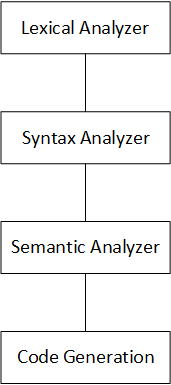
\includegraphics[width=3cm]{images/Diagram.png}
\caption{Structure of a Compiler}
\label{fig_struct_of_compilator}
\end{figure}

\section{Lexical Analyzer}
A lexical analyzer (\textit{Lexer}) is the first front-end step in compilers, matching keywords, comments, operators, etc, and generating a token stream for parsers called \textit{lexemes} consisting of a \textit{token name} and the \textit{attribute value}. 
The \textit{token name} is an abstract symbol that will be used during syntax analysis, while the \textit{attribute value} is an entry in the \textit{symbol table} (discussed on \ref{sub_structure_of_a_compiler}) which will be used during the semantic analysis and the code generation.

The Lexer reads input from the programming language to compile (mini c in our case) and matches it against regular expressions and runs a corresponding action if such an expression is matched.

To make the Lexer are going to use:
\begin{itemize}
	\item Regular Expressions: To describe the lexemes
	\item Finite Automata: To recognize the expressions
\end{itemize}
\subsection{Regular Expressions}
The concept of regular expression arose in the 1950's when the American mathematician Stephen Cole Kleene formalized the description of a regular language.

A regular expression is a sequence of characters that define a search pattern. In other words, there are a conjunction of letters and digits that follow a certain rule.

Let us define \textit{letter} as any letter in the Latin alphabet and \textit{digit} any number [0-9]. Then we can define rules as follow: 
\begin{equation}
0 | [1-9] (<digit>* | [])\label{reg_expr_example}
\end{equation}

Last equation \ref{reg_expr_example} is a declaration of a decimal digit. The "$|$" is a logic or, it means, either the digit is 0 or it will be another thing. If it is not only 0, the number cannot start by 0 in C syntax, so it must start with a digit different from 0, which is range from 1 to 9 (encoded as [0-9]). Secondly, this digit can be followed by either nothing (represented by: []) or by any digit for as many digits are they must be. The format $<$rule$>$* means the repetition of a rule for as many times as necessary, or no repetition at all.

% We could add another example here, for example a comment line or sth.
\subsection{Finite Automata}
A \textit{finite automata} is basically a binary graph which just say "yes" or "no" by means of a \textit{recognizer} to each possible string.

There are two different classes of automatas:
\begin{enumerate}
	\item \textit{Nondeterministic Finite Automata} (NFA)
	\item \textit{Deterministic Finite Automata} (DFA)
\end{enumerate}
The first class (NFA) have no restrictions on the labels of their edges. A symbol can label several edges out of the same state. The DFA on the other hand have for each state and symbol exactly one edge with that symbol leaving that state. 
%translate to english...

\subsection{Implementation}
%The corresponding action will be just to generate an abstract symbol (normally called "token name") that can be read by the next phase (Syntax Analyzer).

For the lexical analyzer, a flex library was used \cite{JFLEX}. A .flex file was created and then, by means of jflex, converted to the final java class.

Jflex lexers are based on a DFA automata. For more information about jflex library please refer to \cite{JFLEX_MANUAL}. 

\section{Syntax Analyzer}

The syntax of a programming language describes the proper form of its programs.

The \textit{syntax analyzer} or \textit{parser} uses the first component of the \textit{lexemes}, the \textit{tokens}. The \textit{parser} creates some kind of tree representation that depicts the grammatical structure of the token stream called the \textit{suntax tree}. In this tree, each node represent an operation and the children of the node represent the arguments of that operation. 

\begin{figure}[H]
	\centering
	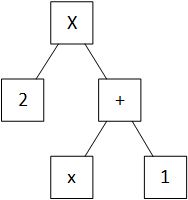
\includegraphics[width=3cm]{images/syntax_tree.png}
	\caption{Syntax Tree Example}
	\label{fig_syntax_tree_example}
\end{figure}

On figure \ref{fig_syntax_tree_example} an example of a tree representation can be seen. Many syntaxes can be the cause of that tree, for example, both \ref{(2*((x)+1))} and \ref{2*(x+1)} can be used to generate such tree.

\begin{equation}
2*(x+1)
\label{2*(x+1)}
\end{equation}

\begin{equation}
(2*((x)+1))
\label{(2*((x)+1))}
\end{equation}

\subsection{Implementation}

The Syntax Analyzer was done using CUP, a parser generator for java \cite{CUP}.

In that file, precedence where applied to each operator using the following table:
\begin{table}[H]
	\begin{center}
	\begin{tabular}{||c c||}
		\hline
		Operator & Associativity  \\ [0.5ex] 
		\hline\hline
		= & right \\ 
		\hline
		$|$$|$ & left  \\
		\hline
		\&\& & left  \\
		\hline
		== != & left  \\
		\hline
		$<$ $<$= $>$ $>$= & left \\ [1ex] 
		\hline
		+ - & left \\
		\hline
		* / & left \\
		\hline
		! -(negative) & right \\
		\hline
		-$>$ & left \\
		\hline
	\end{tabular}
	\end{center}
	\caption{Precedence} \label{tab_precedence}
\end{table}

The higher the operator is in the table, the last will it be applied. For example, the operator "=" will be applied after all the other operators have been applied. There is a very simple way to apply this table in the .cup file by simply writing the following command: precedence <associativity> <token name>. Where associativity is either left or right and the token name is the token from the \textit{lexem} created by the Lexer.

After the precedence, the following grammar was implemented (table \ref{tab_grammar}). The details on how to implement it where omitted. In order to see how to implement the following grammar in cup please refer to the user manual \cite{CUP_MANUAL}.

\begin{table}[H]
	\begin{center}
		\begin{tabular}{ | m{1.5cm} | m{6.5cm}| } 
			\hline
			$<$ file $>$ & $<$ decl $>$* EOF \\ 
			\hline
			$<$ decl $>$ & $<$ var $>$ $|$ $<$ type $>$ $|$ $<$ funct $>$ \\ 
			\hline
			$<$ var $>$ & int $<$ ident $>^{+},$ ; \newline 
						struct $<$ ident $>$ ( *$<$ ident $>^{+},$ ) ; \\ 
			\hline
			$<$ type $>$ & struct $<$ ident $>$ { $<$ var $>$* } ; \\
			\hline
			$<$ funct $>$ & int $<$ ident $>$ ( $<$ param $>^{*},$ ) $<$ bloc $>$ \newline 
							struct $<$ ident $>$ * $<$ ident $>$ ($<$ param $>^{*},$) $<$ bloc $>$ \\
			\hline
			$<$ param $>$ & int $<$ ident $>$ $|$ struct $<$ ident $>$ * $<$ ident $>$ \\
			\hline
			$<$ expr $>$ & 	$<$ integer $>$ \newline 
							$<$ ident $>$ \newline
							$<$ expr $>$ -$>$ $<$ ident $>$ \newline
							$<$ ident $>$ ( $<$ expr $>^{*},$ ) \newline 
							! $<$ expr $>$ $|$ -$<$ expr $>$ \newline
							$<$ expr $>$ $<$ op $>$ $<$ expr $>$ \newline
							sizeof ( struct $<$ ident $>$ ) \newline
							( $<$ expr $>$ )	\\
			\hline
			$<$ op $>$ & = $|$ == $|$ != $|$ + $|$ - $|$ * $|$ / $|$ \&\& $|$ $<$ $|$ $<$= $|$ $>$ $|$ $>$= $|$ $|$$|$ \\ 
			\hline
			$<$ instr $>$ & ; \newline
							$<$ expr $>$; \newline
							if ( $<$ expr $>$ ) $<$ instr $>$\newline
							if ( $<$ expr $>$ ) $<$ instr $>$ else $<$ instr $>$ \newline
							while ( $<$ expr $>$ ) $<$ instr $>$ \newline
							$<$ bloc $>$ \newline
							return $<$ expr $>$; \\				
			\hline
			$<$ instr $>$ & { $<$ var $>*$ $<$ instr $>*$  } \\
			\hline
		\end{tabular}
	\end{center}
	\caption{Grammar} \label{tab_grammar}
\end{table}

Where '$|$' is either one or the other is found. The '*' is as many as necessary (including none at all), while on the other hand, '+' means as many as necessary but at least one. If under any of those symbols there is a comma (',') it means there are comma indented.

Within a file, one will find a list of declarations. These declarations can be either a variable or structure (global variables) of functions. The declarations of functions have it's own parameters (or none) and a bloc in which it will be the code.
The bloc is composed by the declarations of the variables followed by instructions. The instructions are loops such as if or while or simply expressions. Expressions can be all type of C \& C ++ expressions such as integers, pointers, negation, call to functions, etc.   

\section{Semantic Analyzer}
\textit{"Well typed programs do not go wrong"}

The semantics of a programming language defines what each program does when executing.

A \textit{Semantic Analyzer} uses the \textit{syntax tree} and the information in the \textit{symbol table} to check the source program for semantic consistency with the language definition. 

An important part of the \textit{semantic analysis} is the \textit{type checking} where it gathers type information and checks that each operator has matching operands.
An example of the type checking will be to make sure the index which whom an array is accessed is an integer and not any other incompatible type.
In a equation like \(8.0 + 4\), the type checking will make sure to convert the integer "4" into a floating point before making the operation. 

The \textit{type checking} will make sure that the variables of a equation like \(e1 + e2\) are from the same type and reject the incoherent programs. 
There are some languages that use \textbf{dynamic types}, which means they check they check the type of the variables dynamically. Such languages are for example PHP, Python or Lisp. On the other hand, there are also \textbf{static types} languages which is the compiler the one in charge on checking the types. For example OCaml, Java and C (which will be our case).

\section{Code Generation}



\section{Conclusion}

% use section* for acknowledgment
\section*{Acknowledgment}

% Bibliography
\newpage
\IEEEtriggeratref{8}
\bibliographystyle{IEEEtran}
\bibliography{ref}

\end{document}


